\chapter{Projektmanagementplan}

\section{Projektorganisation}

\vspace{1em}

\begin{tabularx}{\textwidth}{|X|X|}
	\hline
	\textbf{Projektbeteiligte} & \textbf{Funktionen} \\
	\hline
	Mike Märki & Stakeholder/Auftraggeber \\
	\hline
	Martin Jud & BDA Experte \\
	\hline
	Pascal Baumann & Product Owner \& Dev Team \\
	\hline
	Dane Wicki & Scrum Master \& Dev Team \\
	\hline
\end{tabularx}

\subsection{Organigramm}
\begin{figure}[h!]
	\centering
	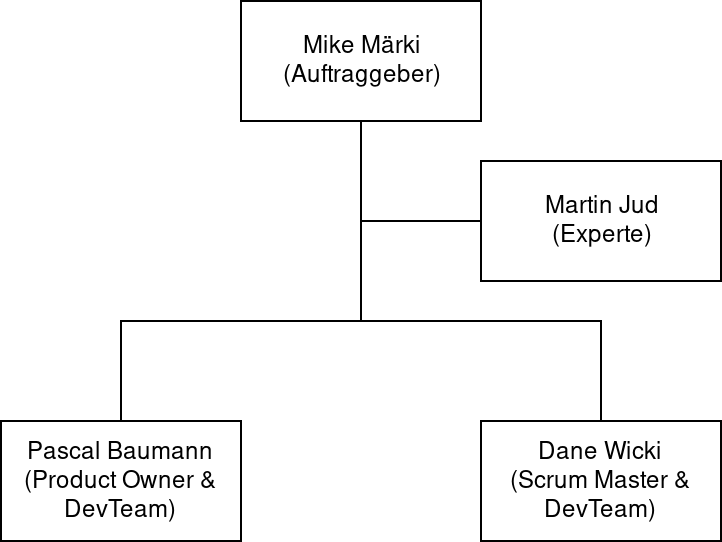
\includegraphics[keepaspectratio, width=0.6\textwidth]{OrganigrammBDA_BAWI.png}
\end{figure}

\subsection{Rollen im Team}
Hier werden die Hauptverantwortlichkeiten des Jeweiligen Teammitgliedes niedergeschrieben. Dies bedeutet nicht, dass dieses jeweilige Mitglied für diese Funktion, Tätigkeit oder Aufgabe alleine zuständig war, sondern lediglich, dass die Entscheidungsgewalt, sowie die Verantwortung bei diesem liegt.

\begin{tabularx}{\textwidth}{|l|X|}
	\hline
	\textbf{Teammitglied} & \textbf{Funktion/Tätigkeit/Aufgaben} \\
	\hline
	Pascal Baumann & Stand der Forschung \\
		& Konzept 2 (Verhinderung des Deplatzieren eines Exemplars) \\
		& Machbarkeitstudie Recherche \\
		& Support Dokumentationssoftware \\
		& Grobplanung \\
		& Risikoanalyse \\
		& CI/CD Dokumentation \\
	\hline
	Dane Wicki & Konzept 1 (Auffindung eines deplatzierten Exemplars)\\
		& Requirements Engineering \\
		& Softwarearchitektur \\
		& Programming Language Advisor \\
		& CI/CD Software \\
		& RFID Hardwarebeschaffung und Verwaltung \\
		& Hardware Interface Specialist \\
		& Sitzungsprotokolle \\
		
	\hline
\end{tabularx}

\section{Rahmenplan}
\subsection{Meilensteine}
\label{ssec:Meilensteine}
Für das Projekt wurden vier Meilensteine definiert, welche jeweils im Vierwochenzyklus auftreten. Diese Meilensteine sind in Abbildung \ref{fig:Milestones} dargestellt.

\begin{figure}[h!]
	\centering
	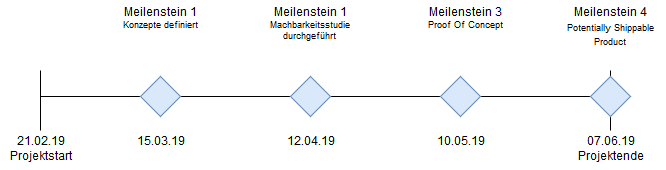
\includegraphics[keepaspectratio,width=0.8\linewidth]{Milestones.png}
	\caption{Die für das Projekt definierten Meilensteine}
	\label{fig:Milestones}
\end{figure}

\subsection{Grobplan}

Aus den im Kapitel \ref{ssec:Meilensteine} definierten Meilensteine wurden acht Sprints von zwei Wochen abgeleitet. In diesen werden sowohl die Artefakte wie Projektdokumentation, Machbarkeitsstudien und Systemspezifikation, wie auch das Produkt entwickelt. Der grobe Rahmenplan ist in Abbildung \ref{fig:Rahmenplan_1} dargestellt.

\begin{figure}[h!]
	\centering
	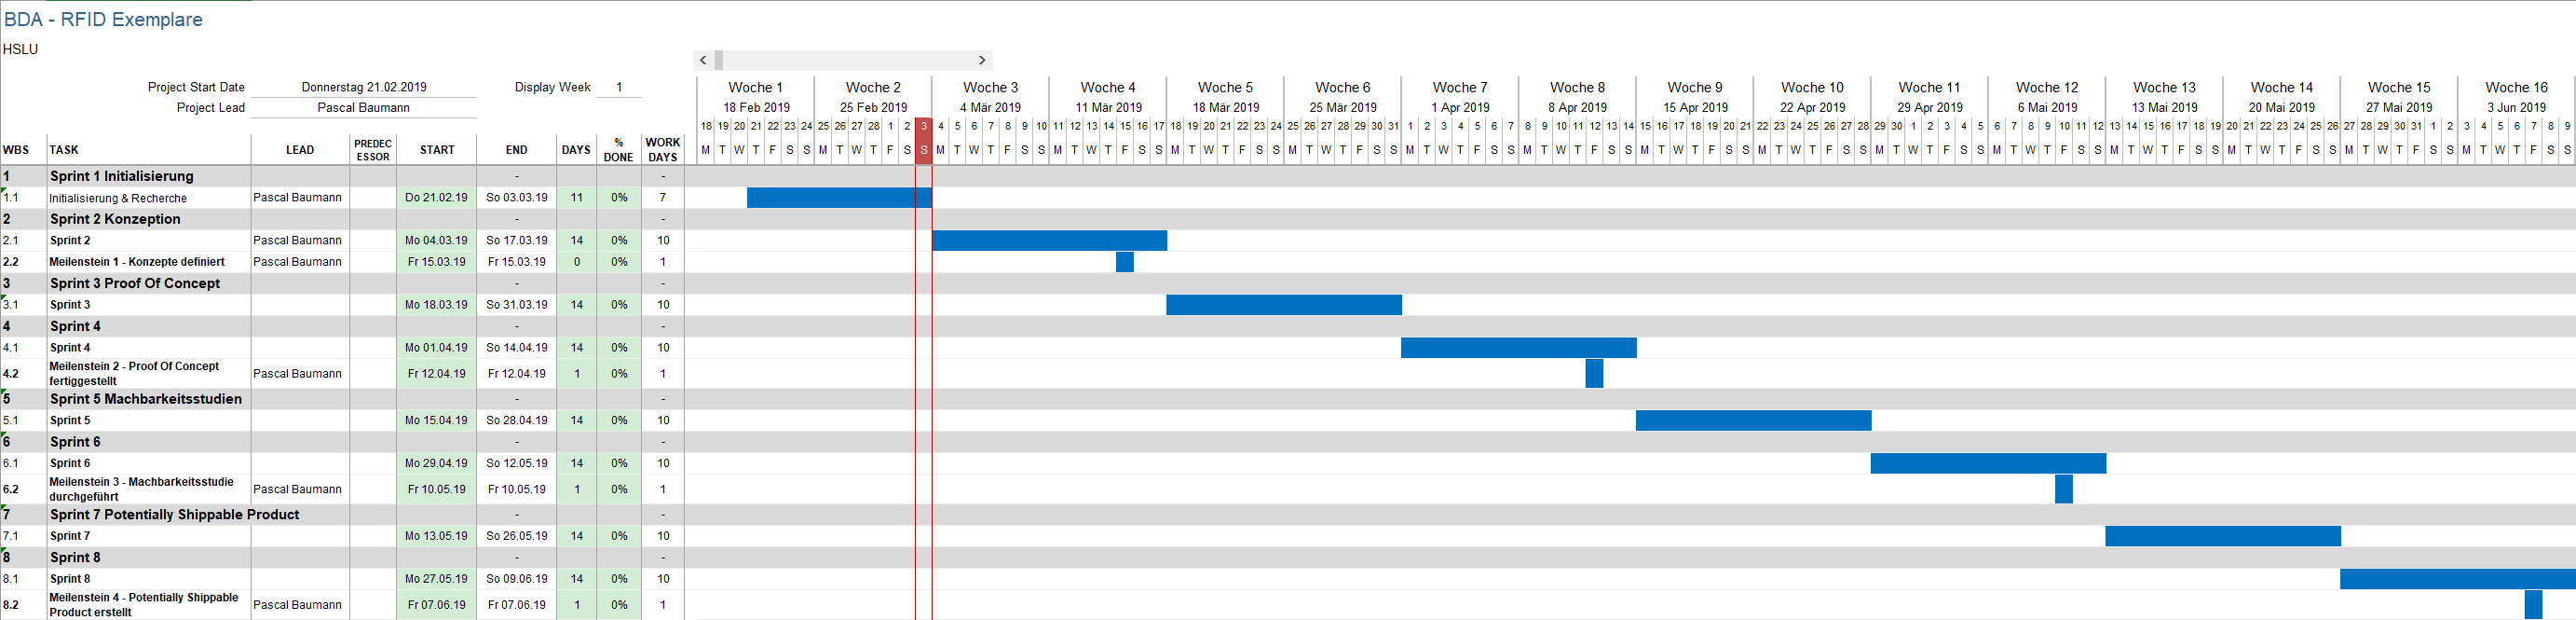
\includegraphics[keepaspectratio,width=\linewidth]{Grobplan.png}
	\caption{Übersicht der Sprints im Rahmenplan}
	\label{fig:Rahmenplan_1}
\end{figure}

\newpage

\section{Tools}
\label{sec:Tools}

\subsection{Versions Kontrolle}
\begin{table}[h!]
	\begin{tabular}{p{0.5\textwidth} p{0.5\textwidth}}
		\hline
		\textbf{Tool} & \textbf{Version} \\
		\hline
		GitKraken & 4.2.2 \\
		\hline
		git & 2.21.0 \\
		\hline
		GitHub & GitHub.com \\
		\hline
	\end{tabular}
	\caption{Verwendete Versionen der Versionierungssysteme}
\end{table}

\subsection{Dokumentation}
\begin{table}[h!]
	\begin{tabular}{p{0.5\textwidth} p{0.5\textwidth}}
		\hline
		\textbf{Tool} & \textbf{Version} \\
		\hline
		TeX Live & 2018 \\
		\hline
		MiKTex & 2.9.6637 \\
		\hline
		Mendeley Desktop & 1.19.2 \\
		\hline
		MS Excel & 16.0.11231.20164 \\
		\hline
	\end{tabular}
	\caption{Verwendete Versionen der Hilfsmittel für die Dokumentation}
\end{table}


\subsection{Repositories \& Buildtools}
\begin{table}[h!]
	\begin{tabular}{p{0.5\textwidth} p{0.5\textwidth}}
		\hline
		\textbf{Name} & \textbf{URL} \\
		\hline
		Dokumentation & \url{https://github.com/HSLU-BaumannWicki/BDA_FS19-Dokumentation} \\
		\hline	
		Travis CI &  \url{https://travis-ci.org/HSLU-BaumannWicki/BDA_FS19-Dokumentation} \\
		\hline
	\end{tabular}
	\caption{Verwendete Repositories}
\end{table}

\subsection{Übrige}
\begin{table}[h!]
	\begin{tabular}{p{0.5\textwidth} p{0.5\textwidth}}
		\hline
		\textbf{Tool} & \textbf{Verwendung} \\
		\hline
		Trello & Aufgabenverwaltung \\
		\hline
		Scrum Poker Online & Storypoints Estimation\\
		\hline
		WhatsApp & Kommunikation im Team \\
		\hline
		OneDrive Online & Dokumentenspeicher \\
		\hline	
	\end{tabular}
	\caption{Übrige Hilfsmittel}
\end{table}

\clearpage

\section{Risikomanagement}

Es werden mögliche Risiken, welche während dem Projekt auftreten können aufgezählt. Diese werden auf Eintrittswahrscheinlichkeit und Schadensmass eingeschätzt, danach wird entschieden, welche Massnahmen getroffen werden können, und was deren Auswirkungen sind.

\subsection{Definitionen}
\label{sssec:Def}
\vspace{1em}
\noindent
Eintrittswahrscheinlichkeit:

\vspace{1em}
\noindent
\begin{tabularx}{\textwidth}{|l|l|X|}
	\hline
	\textbf{Stufe} & \textbf{Bezeichnung} & \textbf{Beschreibung} \\
	\hline
	1 & unvorstellbar & Möglich aber eher unwahrscheinlich. Tritt nie oder einmal in 16 Wochen auf \\
	\hline
	2 & unwahrscheinlich & Kann in 16 Wochen kein oder ein Mal eintreten\\
	\hline
	3 & vorstellbar & Kann in 16 Wochen ein bis zwei Mal eintreten \\
	\hline
	4 & wahrscheinlich & Kann in 16 Wochen bis zu drei Mal eintreten \\
	\hline
	5 & häufig & Kann in 16 Wochen sieben Mal eintreten\\
	\hline
\end{tabularx}

\vspace{1em}
\noindent
Schadensausmass:

\vspace{1em}
\noindent
\begin{tabularx}{\textwidth}{|l|l|X|}
	\hline
	\textbf{Stufe} & \textbf{Bezeichnung} & \textbf{Beschreibung} \\
	\hline
	1 & unwesentlich & Die Aufgabenerfüllung wird höchstens geringfügig beeinträchtigt, finanzieller Schaden ist im Rahmen des Projekts nicht beeinflussend. Personenschäden treten nicht auf. \\
	\hline
	2 & geringfügig & Wahrnehmbare Gefährdung / Einfluss auf das Projekt. Personenschäden treten nicht auf. \\
	\hline
	3 & mittelmässig & Wahrnehmbare Gefährdung / Einfluss auf das Projekt. Verzögerungen zur Folge. Finanzieller Schaden strapaziert das Projektbudget. Personenschäden treten nicht auf. \\
	\hline
	4 & kritisch & Starke Gefährdung des Projekts. Extreme Verzögerungen zur Folge. Finanzieller Schaden übersteigt das Projektbudget. Personenschäden treten geringfügig auf.\\
	\hline
	5 & katastrophal & Projektabbruch zur Folge. Finanzieller Schaden kann zum Projektstopp führen. Verletzung der Persönlichkeitsrechte. \\
	\hline
\end{tabularx}

\newpage

\subsection{Risikokatalog}
\label{sssec:Risikokatalog}
Legende:
\begin{itemize}
	\item \textbf{S}chadensausmass bei Eintreffen des Risikos
	\item \textbf{W}ahrscheinlichkeit das Risiko eintrifft
	\item \textbf{K}ategorie: \textbf{T}echnisches oder \textbf{P}rojektbezogenes Risiko
	\item \textbf{A}uswirkung auf das Projekt. Produkt aus S und W
\end{itemize}

\vspace{1em}
\noindent
\begin{table}[htb]
	\begin{tabularx}{\textwidth}{|l|X|l|l|l||l|}
		\hline
		\textbf{Nr.} & \textbf{Beschreibung / Risiko} & \textbf{K} & \textbf{S} & \textbf{W} & \textbf{A} \\
		\hline
		1 & Meilensteine werden nicht erreicht & P & 4 & 2 & 8 \\
		\hline
		2 & Teammitglied fällt aus & P & 4 & 1 & 4 \\
		\hline
		3 & Fehlkommunikation im Team & P & 4 & 1 & 4 \\
		\hline
		4 & Produkt entspricht nicht den Kundenanforderungen & P & 5 & 2 & 10 \\
		\hline
		5 & Umsetzung des Produkts technisch nicht möglich & T & 3 & 3 & 9 \\
		\hline
		6 & Datenverlust & T & 5 & 2 & 10 \\
		\hline
		7 & Lieferschwierigkeiten von Teilen & P & 3 & 3 & 9 \\
		\hline
		8 & Kosten übersteigen Budgetvorstellung des Kunden & P & 3 & 2 & 6\\
		\hline
		9 & Kosten übersteigen Budgetvorstellung der Hochschule & P & 3 & 3 & 9\\
		\hline
	\end{tabularx}
	\caption{Die im Projekt identifizierten Risiken}
	\label{tbl:Risks}
\end{table}

\vspace{1em}

\begin{figure}[h!]
	\centering
	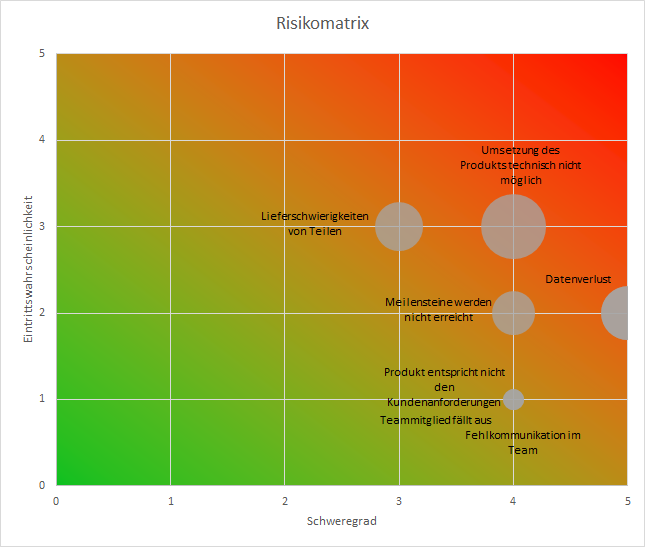
\includegraphics[keepaspectratio, width=0.6\textwidth]{Risks_before.png}
	\caption{Auswirkungen der in Tabelle \ref{tbl:Risks} identifizierten Risiken}
\end{figure}

\newpage

\subsubsection{Massnahmen}

\begin{table}[htb]
	\begin{tabularx}{\textwidth}{|l|X|}
		\hline
		\textbf{Nr.} & \textbf{Beschreibung Massnahme} \\
		\hline
		1 & Meilensteine werden in zwei Zweiwöchigen Sprints absolviert. Die Tasks pro Sprint werden weiter detailliert heruntergebrochen. So sollen die Arbeiten sowohl auf Makro- wie Mikrosicht eingeplant werden. \\
		\hline
		2 & Arbeiten werden so strukturiert und dokumentiert, dass das zweite Mitglied diese auch übernehmen kann. Es werden Spezialisierungen der Teammitglieder insoweit verhindert, dass Wissenslücken minimiert werden. Recherchen sollen Zusammenfassungen und Merkblätter über die gewonnenen Erkenntnisse als Resultat haben.\\
		\hline
		3 & Der Kontakt wird von beiden Teammitgliedern sowohl horizontal im Team wie auch vertikal zu den Stakeholdern aktiv gesucht. Es werden den Arbeiten auch teambildende Aktivitäten zusammen absolviert.\\
		\hline
		4 & Der Kunde muss den Fortschritt alle vier Wochen in einer Sitzung kontrollieren, avisieren und, wenn nötig, Anpassungen fordern.\\
		\hline
		5 & Es soll während den Recherchen schon im Hinblick auf die technische Umsetzung acht gegeben werden.\\
		\hline
		6 & Sowohl produzierten Artefakte, wie auch aktuelle getätigte Arbeiten werden auf auswärtige Plattformen ausgelagert.\\
		\hline
		7 & Teile werden bei Bedarf sofort bestellt, es werden inländische, etablierte Lieferanten, vor evtl. günstigeren Ausländischen vorgezogen.\\
		\hline
		8 & Lösungskonzept wird in der erarbeiteten Form verworfen und durch günstigere Komponenten ersetzt.\\
		\hline
		9 & Es werden alternative Sponsoren von Geldmittel gesucht.\\
		\hline
	\end{tabularx}
	\caption{Massnahmen um Effekte oder Eintrittswahrscheinlichkeit zu reduzieren}
\end{table}

\vspace{1em}

\begin{table}[htb]
	\begin{tabularx}{\textwidth}{|l|X|l|l|l||l|}
		\hline
		\textbf{Nr.} & \textbf{Beschreibung / Risiko} & \textbf{K} & \textbf{S} & \textbf{W} & \textbf{A} \\
		\hline
		1 & Meilensteine werden nicht erreicht & P & 4 & 1 & 4 \\
		\hline
		2 & Teammitglied fällt aus & P & 3 & 1 & 3 \\
		\hline
		3 & Fehlkommunikation im Team & P & 4 & 1 & 4 \\
		\hline
		4 & Produkt entspricht nicht den Kundenanforderungen & P & 5 & 1 & 5 \\
		\hline
		5 & Umsetzung des Produkts technisch nicht möglich & T & 4 & 3 & 12 \\
		\hline
		6 & Datenverlust & T & 5 & 1 & 5 \\
		\hline
		7 & Lieferschwierigkeiten von Teilen & P & 3 & 2 & 6 \\
		\hline
		8 & Kosten übersteigen Budgetvorstellung des Kunden & P & 3 & 1 & 3\\
		\hline
		9 & Kosten übersteigen Budgetvorstellung der Hochschule & P & 3 & 2 & 6\\
		\hline
	\end{tabularx}
	\caption{Neueinschätzung der Risiken nach Einführung der Massnahmen}
	\label{tbl:Massnahmen}
\end{table}

\vspace{1em}

\begin{figure}[h!]
	\centering
	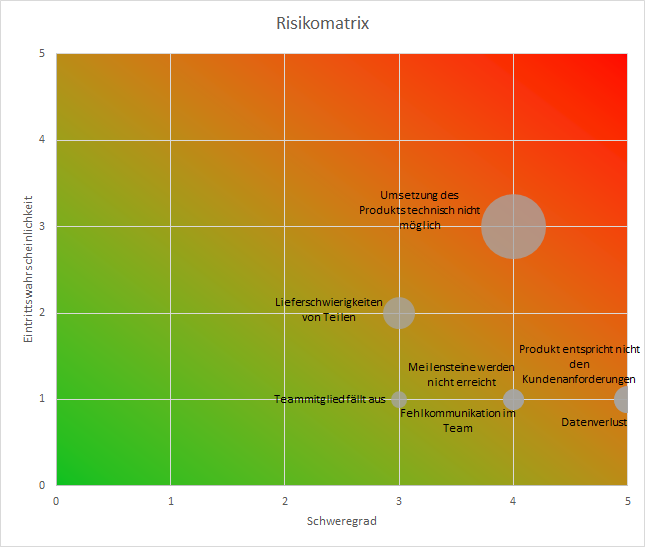
\includegraphics[keepaspectratio, width=0.6\textwidth]{Risks_after.png}
	\caption{Auswirkungen der Risiken nach den in Tabelle \ref{tbl:Massnahmen} vorgeschlagenen Massnahmen}
\end{figure}
